\documentclass[a4paper,12pt]{report} % Paper format

% Packages
%\usepackage[T2A]{fontenc}	% Internal LaTeX fonts table
\usepackage[utf8]{inputenc}	% Encoding of this document
\usepackage[english,russian]{babel}	% Using russian and english dictionaries
\usepackage{amsfonts,amsmath,calc,fancyhdr,geometry,graphicx,indentfirst,latexsym}	% All used packages
\usepackage{totpages}

% СТП СГАУ 6.1.4 - 97
\newlength{\standardleftmargin}	% Absolute left margin
\newlength{\standardrightmargin}	% Absolute right margin
\newlength{\standardtopmargin}	% Absolute top margin
\newlength{\standardbottommargin}	% Absolute bottom margin
\setlength{\standardleftmargin}{30mm}	% Absolute left margin
\setlength{\standardrightmargin}{10mm}	% Absolute right margin
\setlength{\standardtopmargin}{15mm}	% Absolute top margin
\setlength{\standardbottommargin}{20mm}	% Absolute bottom margin

% Nesting
%\pagestyle{fancy}
%\fancyhead{}
%\fancyfoot{}
%\fancyhead[R]{\thepage}
%\fancyhead[C]{Аналитическое решение краевых задач математической физики}
\renewcommand{\baselinestretch}{1.5}	% Sesquialteral interval
\setlength{\hoffset}{\standardleftmargin - 1in - \oddsidemargin}
\setlength{\voffset}{\standardtopmargin - 1in - \topmargin}
\setlength{\textwidth}{\paperwidth - 1in - \hoffset - \oddsidemargin - \marginparsep - \marginparwidth - \standardrightmargin}
\setlength{\textheight}{\paperheight - 1in - \voffset - \topmargin - \headheight - \headsep - \footskip - \standardbottommargin}
\setlength{\headwidth}{\textwidth + \marginparsep + \marginparwidth}

% \addto\captionsrussian{\def\refname{Использованные источники}}

% Macro

\makeatletter
\renewcommand{\@makechapterhead}[1]{
  \vspace*{50 pt}
  {\parindent=0pt
   \raggedright \normalfont\huge\bfseries
   \@chapapp{}
    \normalfont\Huge\bfseries \thechapter ~ #1\par
    \nopagebreak
    \vspace{40 pt}
  }
}
\makeatother

% Commands

\newcommand{\diff}{\mathrm{d}}

\newenvironment{equationsset}
{\left\{\begin{array}{rcl}}
{\end{array}\right.}

% Long formulas
\allowdisplaybreaks


% Page properties
\author{Caesar}	% Author
\title{Рассчётная работа}	% Title
\begin{document}
\renewcommand{\chaptername}{}
\input{CoverPage}
\input{Problem}
\input{Summary}

\renewcommand{\contentsname}{\begin{center}Содержание\end{center}}

\newcommand{\tocsecindent}{\hspace{7mm}}
\renewcommand\bibname{Список использованных источников}

%Page numbers
\setcounter{page}{2}
\tableofcontents
%\input{Introduction}

% Body
\chapter*{Введение}
\addcontentsline{toc}{chapter}{\tocsecindent{Введение}}

В данной работе решается краевая задача математической физики, основанная на волновом уравнении, и программно моделируется распространение поляризованной электромагнитной волны в плоскопараллельном однородном волноводе. Подобные задачи возникают при исследовании электромагнитных волн, построении волноводов, передающих сигналы.

Для их решения применяются различные методы: аналитические, численные, вариационные, проекционные.  В данной работе рассматриваются аналитические методы, в частности для решения предложенной задачи используется метод Фурье разделения переменных. Этот метод выбран ввиду того, что сама задача линейна относительно частных производных с постоянными коэффициентами, а метод Фурье прост для понимания и предназначен как раз для решения таких задач.

Схема решения заключается в следующем: искомая функция факторизуется по каждому своему параметру, затем решается задача Штурма-Лиувилля и получаются собственные функции оператора Лапласа. Далее решение ищется в виде ряда по этим собственным функциям.

Для наглядности написана программа, анимирующая распространение электромагнитной волны в волноводе на основе полученного решения. Кроме того, получена равномерная оценка погрешности вычислений и проведено исследование её эффективности.
\chapter{Математическая модель}

Из уравнений Максвелла получаем общий вид волнового уравнения:

\begin{equation}
\label{eq:wave_equation}
\Delta \vec{E} = \frac{1}{a^2} \frac{\partial^2 \vec{E}}{\partial t^2} + \frac{4 \pi \sigma \mu}{c^2} \frac{\partial \vec{E}}{\partial t},
\end{equation}

\begin{tabbing}
где \= $\Delta = \frac{\partial^2}{\partial x^2} + \frac{\partial^2}{\partial y^2} + \frac{\partial^2}{\partial z^2}$ \=~--- оператор Лапласа,\\
\> $\sigma$ \>~--- электрическая проводимость среды,\\
\>$\varepsilon$ \>~--- диэлектрическая проницаемость среды,\\
\>$\mu$ \>~--- магнитная проводимость среды,\\
\>$a = \frac{c}{\varepsilon \mu}$ \>~--- скорость распространения электромагнитных волн в среде.
\end{tabbing}

Вывод \eqref{eq:wave_equation} из уравнений Максвелла можно найти, например в \cite{samarsky}.

Преобразуем \eqref{eq:wave_equation} для нашего случая. Положим, что внутри волновода вакуум, а стенки его по условию изготовлены из проводящего материала. В вакууме $\sigma = 0$, $\varepsilon = 1$, $\mu = 1$, а значит $a = c$. Кроме того, в нашем случае $\vec{E} = \left( E_x, 0, 0\right)$, т.~е. нам нужно рассматривать \eqref{eq:wave_equation} только в проекции на одну координату $E_x$. Причем $E_x$ по условию зависит только от $y$, $z$ и $t$, а от $x$ не зависит. Значит и $\frac{\partial^2 E_x}{\partial x^2} = 0$.

С учетом этого, \eqref{eq:wave_equation} перепишется в виде

\begin{equation}
\label{eq:wave_equation_2}
\Delta_{yz} E_x = \frac{1}{c^2} \frac{\partial^2 E_x}{\partial t^2}.
\end{equation}

Здесь использовано довольно распространенное обозначение $\Delta_{xy} = \frac{\partial^2}{\partial y^2} + \frac{\partial^2}{\partial z^2}$.

Задумаемся о краевых условиях для нашей задачи. Раз три стенки выполнены из электропроводящего матриала, значит на них напряженности поля никогда не возникнет: $\left. E_x \right|_{y=0} = \left. E_x \right|_{y=l_y} = \left. E_x \right|_{z=l_z} = 0$. Напряженность на оставшейся стенке нам известна. Она поддерживается неким источником и изменяется по известному закону: $\left. E_x \right|_{z=0} = \sin\frac{\pi y}{l_y} \sin\frac{2 \pi c}{\lambda}t$ все интересующее нас время. При этом в начальный момент времени на всем волноводе какая-либо напряженность отсутствует и ее производная во времени --- тоже: $\left. E_x \right|_{t=0} = \left. \frac{\partial E_x}{\partial t} \right|_{t=0} = 0$. Присовокупив к \eqref{eq:wave_equation_2} эти условия, получим задачу математической физики:

\begin{equation}
\label{eq:problem}
\left\{
\begin{array}{rclr}
\frac{1}{c^2} \frac{\partial^2 E_x}{\partial t^2} &=& \Delta_{yz} E_x, & 0 \le y \le l_y, 0 \le z \le l_z, 0 \le t \le T; \\
\left. E_x \right|_{y=0} & = & 0, & 0 < z < l_z, 0 < t \le T; \\
\left. E_x \right|_{y=l_y} & = & 0, & 0 < z < l_z, 0 < t \le T; \\
\left. E_x \right|_{z=0} &=&  \sin\frac{\pi y}{l_y} \sin\frac{2 \pi c}{\lambda} t, & 0 \le y \le l_y, 0 < t \le T; \\
\left. E_x \right|_{z=l_z} &=& 0, & 0 \le y \le l_y, 0 < t \le T; \\
\left. E_x \right|_{t=0} & = & 0, & 0 \le y \le l_z, 0 \le z \le l_z; \\
\left. \frac{\partial E_x}{\partial t} \right|_{t=0} &=& 0, & 0 \le y \le l_z, 0 \le z \le l_z.
\end{array}
\right.
\end{equation}

Как видно, задачу \eqref{eq:problem} невозможно решить методом разделения переменных вследствие неоднородного краевого условия. Для решения этой
проблемы сделаем замену $U(y, z, t) = E_x(y, z, t) - \frac{l_z - z}{l_z} \sin\frac{2 \pi c}{\lambda}t \sin\frac{\pi y}{l_y}$. Получим следующую задачу
математической физики:

\begin{equation}
\label{eq:new_problem}
\left\{
\begin{array}{rclr}
\frac{1}{c^2} \frac{\partial^2 U}{\partial t^2} & = & \Delta_{yz} U + G(y, z, t), & 0 \le y \le l_y, 0 \le z \le l_z, 0 \le t \le T; \\
\left. U \right|_{y=0} & = & 0, & 0 < z < l_z, 0 < t \le T; \\
\left. U \right|_{y=l_y} & = & 0, & 0 < z < l_z, 0 < t \le T; \\ 
\left. U \right|_{z=0} & = &  0, & 0 \le y \le l_y, 0 < t \le T; \\
\left. U \right|_{z=l_z} &=& 0, & 0 \le y \le l_y, 0 < t \le T; \\
\left. U \right|_{t=0} & = & 0, & 0 \le y \le l_z, 0 \le z \le l_z; \\
\left. \frac{\partial U}{\partial t} \right|_{t=0} &=& \Phi(y, z), & 0 \le y \le l_z, 0 \le z \le l_z.
\end{array}
\right.
\end{equation}

Здесь сразу же для компактности записи использованы обозначения:

\begin{equation}
\label{eq:g}
G(y, z, t) = \pi^2 c^2\frac{l_z - z}{lz}\frac{4l_y^2 - \lambda^2}{\lambda^2 \l_y^2}\sin k t \sin\frac{\pi y}{l_y},
\end{equation}

\begin{equation}
\label{eq:phi}
\Phi(y, z) = -k\frac{l_z - z}{l_z}\sin\frac{\pi y}{l_y},
\end{equation}

\begin{equation}
\label{eq:k}
k = \frac{2 \pi c}{\lambda}.
\end{equation}


Получена неоднородная задача, имеющая однородные краевые условия, что
позволяет нам применять метод разделения переменных.

\chapter{Решение}
\section{Собственные функции}
Для последующих действий необходимо представить функцию $U$ из задачи \eqref{eq:new_problem} в виде разложения по собственным функциям. Сначала найдем собственные функции. Для этого решим задачу Штурма-Лиувилля.\\
Представим функцию $U$ в форме  
\begin{equation}
  \label{func:form}
  U(y, z, t) = T(t)Y(y)Z(z).
\end{equation}

Рассмотрим однородное уравнение
\begin{equation}
  \label{eq:uniform}
  \frac{1}{c^2} \frac{\partial^2 U}{\partial t^2} = \Delta_{yz} U.\\
\end{equation}

Подставив \eqref{func:form} в \eqref{eq:uniform}, получим
\begin{equation}
  \label{eq:equality}
  \frac{1}{c^2}\frac{T''}{T} = \frac{Y''}{Y} + \frac{Z''}{Z} = -(\lambda^2 + \mu^2).\\
\end{equation}

Здесь $\lambda^2 = \const, \mu = \const$ в силу того, что левая часть \eqref{eq:equality} зависит только от $t$,
а правая~--- от $y$ и $z$. Отсюда следует, что
\begin{equation}
  \label{eq:shturm-liuville}
  \left.
  \begin{array}{rcl}
    Y'' + \lambda^2 Y &=& 0,\\
    Z'' + \mu^2 Z &=& 0,\\
    T'' + c^2(\lambda^2 + \mu^2)T &=& 0.
  \end{array}
  \right.
\end{equation}

Подставив, кроме того, \eqref{func:form} в граничные условия \eqref{eq:new_problem} получим условия
\begin{equation}
  \left.
  \label{eq:conditions}
  \begin{array}{rcl}
    Y(0) &=& 0,\qquad Y(l_y) = 0,\\
    Z(0) &=& 0,\qquad Z(l_y) = 0.
  \end{array}
  \right.
\end{equation}

Таким образом, использовав \eqref{eq:shturm-liuville} и \eqref{eq:conditions}, мы получим две задачи о собственных значениях (задачи Штурма-Лиувилля) для $Y$ и $Z$.
\begin{equation}
  \label{eq:shturm-liuville-final}
  \begin{array}{ll}
    \left\{
      \begin{array}{l}
        Y'' + \lambda^2Y = 0, \\
        Y(0) = Y(l_y) = 0;
      \end{array}
    \right.
    \left\{
      \begin{array}{l}
        Z'' + \mu^2Z = 0, \\
        Z(0) = Z(l_z) = 0.
      \end{array}
    \right.  
  \end{array}
\end{equation}

Решим первую задачу из системы \eqref{eq:shturm-liuville-final}. Как известно (см. \cite{samarsky}) общее решение такого уравнения представимо в виде
\begin{equation}
  \label{eq:common-solution}
  Y(y) = A\sin{\lambda y} + B\cos{\lambda y}.
\end{equation}

Первое граничное условие $Y(0) = 0$ дает нам $B = 0$. Из второго условия $Y(l_y) = 0$ следует 
\[
Y(l_y) = A\sin{\lambda l_y} = 0.
\]

Поскольку $Y(y)$ не равно тождественно нулю, то $A \ne 0$, значит
\begin{equation}
  \label{eq:sin}
  \sin{\lambda l_y} = 0.
\end{equation}

Из \eqref{eq:sin} следует, что $\lambda = \cfrac{\pi n}{l_y}$.

Аналогично решаем вторую задачу системы \eqref{eq:shturm-liuville-final} и получаем нетривиальные решения
\begin{equation}
  \label{func:eigen}
  \begin{array}{ll}
    \left\{
      \begin{array}{l}
        Y = A\sin\lambda y, \\
        \lambda = \frac{\pi n}{l_y},
      \end{array}
    \right.
    \left\{
      \begin{array}{l}
        Z = B\sin\mu z, \\
        \mu = \frac{\pi m}{l_z}.
      \end{array}
    \right.  
  \end{array}
\end{equation}

\section{Получение решения}

Таким образом, $U$ можно представить в виде следующего двойного ряда Фурье по функциям \eqref{func:eigen}.
\begin{equation}
  \label{eq:u-series}
  U(y, z, t) = \displaystyle \sum_{m=1}^{\infty}\sum_{n=1}^{\infty} \gamma(t) \sin\frac{\pi n y}{l_y} \sin\frac{\pi m z}{l_z}.
\end{equation}
\\
Разложим собственным функциям \eqref{func:eigen} неоднородную правую часть $G(y, z, t)$ системы \eqref{eq:new_problem} и функцию $\Phi(y, z)$. В дальнейших рассуждениях для простоты умножим левую и правую части первого уравнения \eqref{eq:new_problem} на $c^2$, получив
\begin{equation}
  \label{eq:new_eq_simple}
  \frac{\partial^2 U}{\partial t^2} = \Delta_{yz} U + c^2G(y, z, t)
\end{equation}

\begin{enumerate}
\item Разложение $G(y, z, t)$.
  Разложим функцию $G(y, z, t) = \pi^2 c^2\frac{l_z - z}{lz}\frac{4l_y^2 - \lambda^2}{\lambda^2 \l_y^2}\sin\frac{2\pi c}{\lambda}t \sin\frac{\pi y}{l_y}$ по функциям \eqref{func:eigen}. Заметим, что функция $G$ уже содержит в себе собственную функцию $\sin\frac{\pi y}{l_y}$, значит, необходимо разложить лишь зависящую от $z$ часть. Разложение будет иметь вид
  \begin{equation}
    \label{func:G_represent}
    G(y, z, t) =  \pi^2 c^2 \frac{4l_y^2 - \lambda^2}{\lambda^2 \l_y^2} \sin\frac{2\pi c}{\lambda}t\displaystyle \sum_{m=1}^{\infty}  g_{nm}^{(z)}(t) \sin\frac{\pi y}{l_y} \sin\frac{\pi m z}{l_z}.
  \end{equation}
  Найдем коэффициенты ряда.
%   \begin{equation}
%     \label{func:g}
%     \begin{array}{rcl}
%       g^{(z)}_{nm}(t) &=& \frac{2}{l_z} \displaystyle \int_0^{l_z} \frac{l_z - z}{l_z} \sin\frac{\pi m z}{l_z} dz
%       =\frac{2}{l_z}\left[\int_0^{l_z}\sin\frac{\pi m z}{l_z}dz - \int_0^{l_z}\frac{z}{l_z} \sin\frac{\pi m z}{l_z}dz\right] =\\
%       \\
%       &=& \frac{2}{l_z} \left[ \left. -\frac{l_z}{\pi m} \cos\frac{\pi m z}{l_z}\right|_{0}^{l_z} - \left. \frac{z l_z}{\pi m}\cos\frac{\pi m z}{l_z}\right|_{0}^{l_z} + \int_0^{l_z}\frac{l_z}{\pi m}\cos\frac{\pi m z}{l_z}dz\right] =\\
%       \\
%       &=& \frac{2}{l_z}\frac{l_z}{\pi m} \left( 1 - (-1)^m - (-1)^{m+1} \right) = \frac{2}{\pi m}.
%     \end{array}
%   \end{equation}
  \begin{eqnarray}
    \nonumber
    g^{(z)}_{nm}(t) &=& \frac{2}{l_z} \displaystyle \int_0^{l_z} \frac{l_z - z}{l_z} \sin\frac{\pi m z}{l_z} dz = \frac{2}{l_z}\left[\int_0^{l_z}\sin\frac{\pi m z}{l_z}dz - \int_0^{l_z}\frac{z}{l_z} \sin\frac{\pi m z}{l_z}dz\right] =\\
    \nonumber
    &=& \frac{2}{l_z} \left[ \left. -\frac{l_z}{\pi m} \cos\frac{\pi m z}{l_z}\right|_{0}^{l_z} - \left. \frac{z l_z}{\pi m}\cos\frac{\pi m z}{l_z}\right|_{0}^{l_z} + \int_0^{l_z}\frac{l_z}{\pi m}\cos\frac{\pi m z}{l_z}dz\right] =\\
    \label{func:g}
    &=& \frac{2}{l_z}\frac{l_z}{\pi m} \left( 1 - (-1)^m - (-1)^{m+1} \right) = \frac{2}{\pi m}.
  \end{eqnarray}
  
  Подставив разложение \eqref{func:g} в \eqref{func:G_represent} получим
  \begin{equation}
    \label{func:G}
    G(y, z, t) = 2\pi c^2\frac{4l_y^2 - \lambda^2}{\lambda^2 \l_y^2} \sin\frac{2\pi c}{\lambda}t\displaystyle \sum_{m=1}^{\infty}\frac{1}{m}\sin\frac{\pi y}{l_y} \sin\frac{\pi m z}{l_z}.
  \end{equation}

\item Разложение начального условия.


  Для удобства введем замену $k = \frac{2\pi c}{\lambda}$. Теперь разложим начальное условие  $\Phi(y, z, t) = -k\frac{l_z - z}{l_z}\sin\frac{\pi y}{l_y}$. Как и в предыдущем случае, она уже разложена по собственным функциям относительно $y$, будем искать разложение относительно $sin\frac{\pi m z}{l_z}$. Разложения будет иметь следующий вид
  \[
  \Phi(y, z, t) = \displaystyle -k\sum_{m=1}^{\infty}\varphi(t) \sin\frac{\pi y}{l_y} \sin\frac{\pi m z}{l_z}.
  \]
  Найдем коэффициенты разложения
  \begin{eqnarray*}
    \varphi(t) = \displaystyle \frac{2}{l_z} \int_0^{l_z} \frac{l_z - z}{l_z}\sin\frac{\pi m z}{l_z}dz = \frac{2}{\pi m}.
  \end{eqnarray*}
  Таким образом
  \[
  \Phi(y, z, t) = -\frac{2k}{\pi}\displaystyle \sum_{m=1}^{\infty} \frac{1}{m} \sin\frac{\pi y}{l_y} \sin\frac{\pi m z}{l_z}.
  \]
\end{enumerate}

Подставим все полученные разложения и учтем, что правая часть и начальное условие не являются нулевыми лишь при $n = 1$, поэтому и разложение $U(y, z, t)$ представим в виде обыкновенного ряда Фурье.
\[
U(y, z, t) = \displaystyle \sum_{m=1}^{\infty} \gamma(t) \sin\frac{\pi y}{l_y} \sin\frac{\pi m z}{l_z}.
\]
Подставив в систему разложения и приравняв коэффициенты при одинаковых базисных функциях, получим систему обыкновенных дифференциальных уравнений с начальными условиями вида
\[
\left\{
    \begin{array}{l}
      \gamma''(t) + w^2_{m}\gamma(t) = \frac{2\pi c^2}{m}\left(\frac{4l_y^2 - \lambda^2}{l_y^2\lambda^2} \right)\sin{kt},\\
      \begin{array}{rcl}
      \gamma(0) &=& 0,\\
      \gamma'(0) &=& -\frac{2k}{\pi m}.
      \end{array}
    \end{array}
\right.
\]\\
Здесь $w_{m} = \pi c \sqrt{\frac{1}{l_y^2} + \frac{m^2}{l_z^2}}$\\
Найдем общее решение соответствующего однородного уравнения
\[
\begin{array}{l}
  \gamma''(t) + w^2_{m}\gamma(t) = 0,\\
  \gamma^{0}(t) = A\cos{w_m t} + B\sin{w_mt}.
\end{array}
\]
Рассмотрим теперь неоднородную задачу и найдем ее частное решение. Исходя из вида правой части, вид решения будет таким
\[
\tilde{\gamma}(t) = C\cos{kt} + D\sin{kt}.
\]
Подставим функцию такого вида в уравнение и получим
\[
-k^2C\cos{kt} - k^2 D\sin{kt} + w^2_m C\cos{kt} + w^2_{m} D\cos{kt} = \frac{2\pi c^2}{m}\left(\frac{4l_y^2 - \lambda^2}{l_y^2\lambda^2} \right)\sin{kt}.
\]
Приравняем коэффициенты при соответствующих функциях и получим систему
$\begin{equationsset}
      (w_m^2 - k^2)C & = & 0, \\
      (w_m^2 - k^2)D & = & \frac{2\pi c^2}{m}\left(\frac{4l_y^2 - \lambda^2}{l_y^2\lambda^2} \right).
\end{equationsset}$
      

Отсюда $C = 0$, $D = \frac{2\pi c^2}{m(w_m^2 - k^2)}\left(\frac{4l_y^2 - \lambda^2}{l_y^2\lambda^2} \right)$.\\
Общее решение выглядит как сумма общего решения однородного уравнения и частного решения неоднородного, то есть
\[
\gamma(t) = A\cos{w_mt} + B\sin{w_mt} + \frac{2\pi c^2}{m(w_m^2 - k^2)}\left(\frac{4l_y^2 - \lambda^2}{l_y^2\lambda^2} \right)\sin{kt}.
\]
Используем начальные условия и получим систему
\[
\left\{
  \begin{array}{l}
    A = 0,\\
    w_nB + kD = -\frac{2k}{\pi m} \Rightarrow B = -\frac{k}{w_m}\left(\frac{2}{\pi m} + D \right).
  \end{array}
\right.
\]
Таким образом,
\begin{eqnarray*}
  \gamma(t) &=& \frac{2\pi c^2}{m(w_m^2 - k^2)}\left(\frac{4l_y^2 - \lambda^2}{l_y^2\lambda^2} \right)\sin{kt} - \frac{k}{w_m}\left(\frac{2}{\pi m} + D\right)\sin{w_mt},\\
  U(y, z, t) &=& \displaystyle \sum_{m=1}^{\infty} \left( \frac{2\pi c^2}{m(w_m^2 - k^2)}\left(\frac{4l_y^2 - \lambda^2}{l_y^2\lambda^2} \right)\sin{kt} - \frac{k}{w_m}\left(\frac{2}{\pi m} + D\right)\sin{w_mt} \right) \sin\frac{\pi y}{l_y} \sin\frac{\pi m z}{l_z},\\
  E_x(y, z, t) &=& \displaystyle
    \sum_{m=1}^{\infty} \left( \frac{2\pi c^2}{m(w_m^2 - k^2)}\left(\frac{4l_y^2 - \lambda^2}{l_y^2\lambda^2} \right)\sin{kt} - \frac{k}{w_m}\left(\frac{2}{\pi m} + D\right)\sin{w_mt} \right) \sin\frac{\pi y}{l_y} \sin\frac{\pi m z}{l_z}\\
    &+& \frac{l_z - z}{l_z} \sin\frac{2\pi c}{\lambda}t \sin\frac{\pi y}{l_y}
\end{eqnarray*}

\begin{figure}[!hbtp]
  \center
  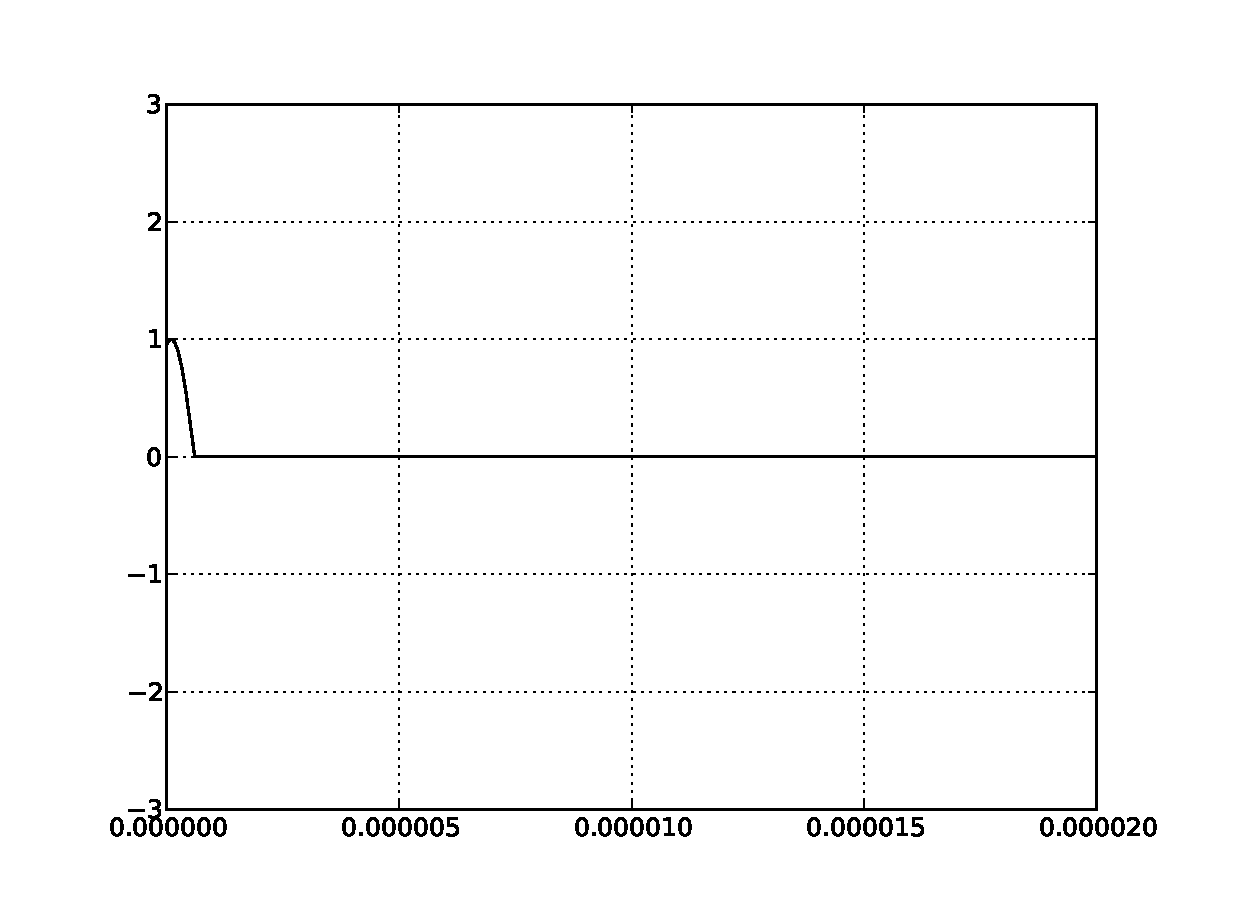
\includegraphics[width=0.9\linewidth]{first}
  \caption{Волна в момент $t = 2\cdot10^{-15}$}
\end{figure}

\begin{figure}[!hbtp]
  \center
  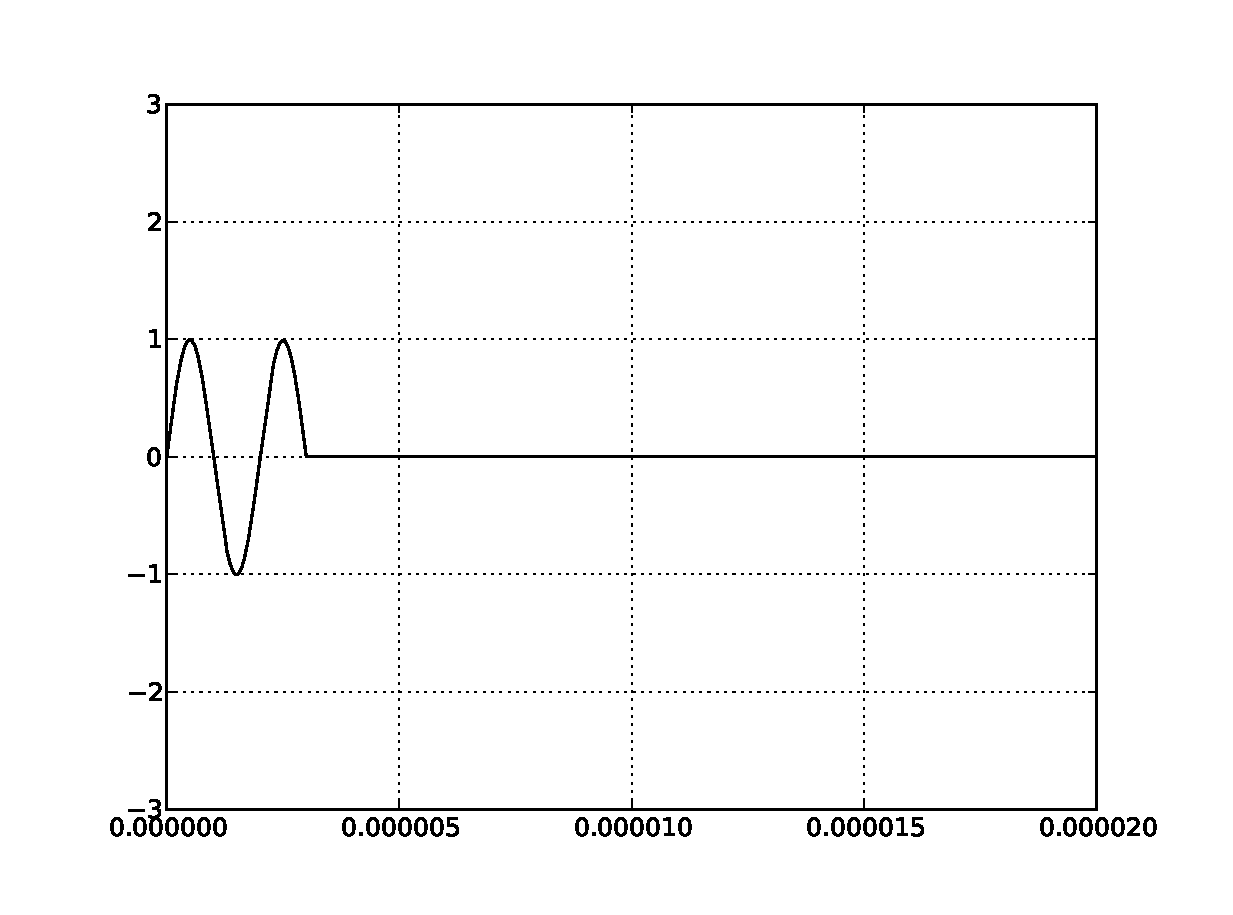
\includegraphics[width=0.9\linewidth]{second}
  \caption{Волна в момент $t = 1\cdot10^{-14}$}
\end{figure}

\begin{figure}[!hbtp]
  \center
  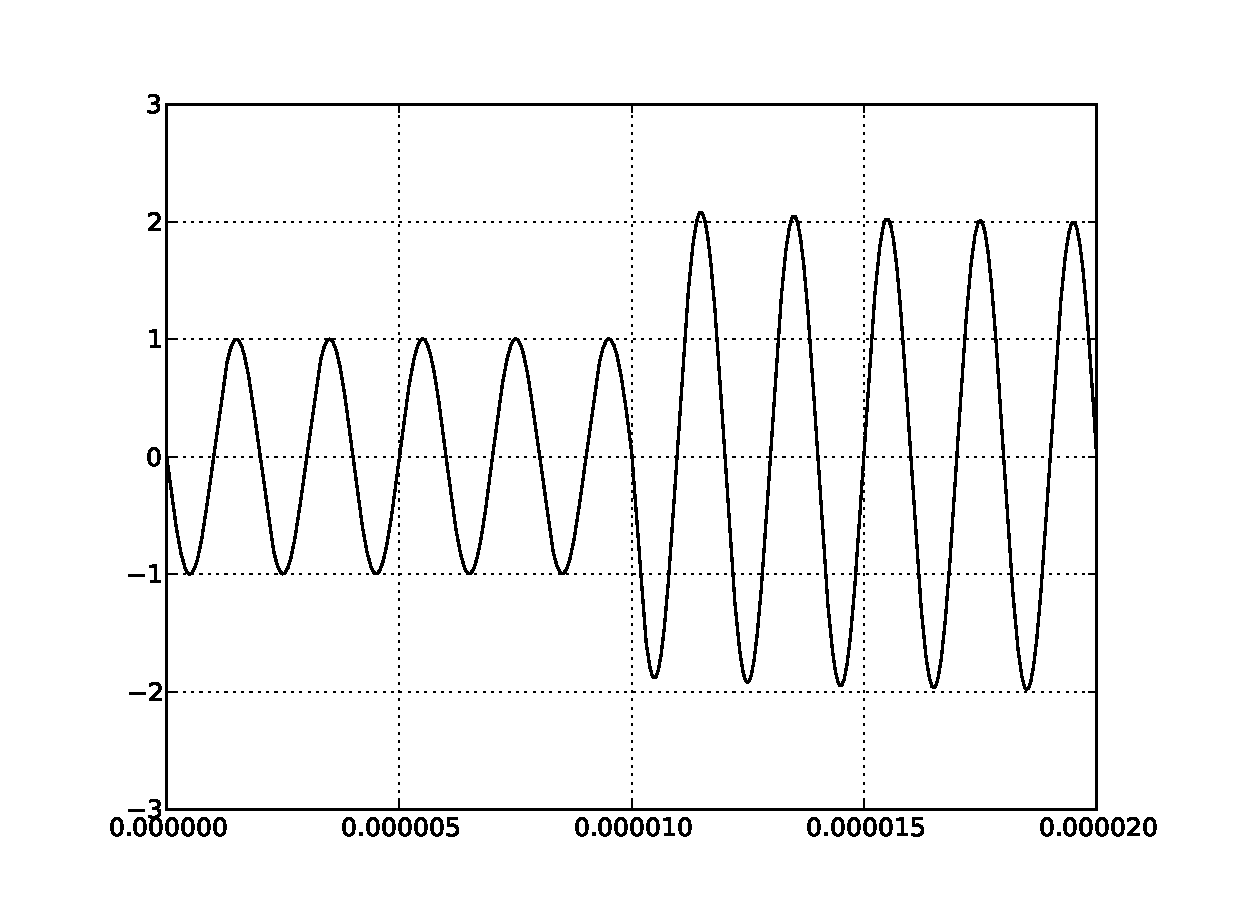
\includegraphics[width=0.9\linewidth]{third}
  \caption{Волна в момент $t = 1\cdot10^{-13}$}
\end{figure}

\chapter{Исследование сходимости}
\section{Оценка погрешности}

Итак, мы получили решение в виде ряда. Чтобы выдавать численное значение напряжённости, нам необходимо суммировать определённое конечное количество элементов ряда. Пусть это будет $M$ элементов.
\begin{eqnarray*}
&&S_M = \sum \limits_{m=1}^{M} \left( \frac{2\pi c^2}{m(w_m^2 - k^2)}\left(\frac{4l_y^2 - \lambda^2}{l_y^2\lambda^2} \right)\sin{kt} - \frac{k}{w_m}\left(\frac{2}{\pi m} + D\right)\sin{w_mt} \right) \sin\frac{\pi y}{l_y} \sin\frac{\pi m z}{l_z}.\\
\end{eqnarray*}

Эту частичную сумму мы и будем выдавать в качестве ответа. При этом мы ошибёмся на величину, равную модулю хвоста ряда, начиная с $(M+1)$-ого элемента. Обозначим за $r_M$ хвост нашего ряда.
\[
r_M = \sum \limits_{m=M+1}^{\infty} \left( \frac{2\pi c^2}{m(w_m^2 - k^2)}\left(\frac{4l_y^2 - \lambda^2}{l_y^2\lambda^2} \right)\sin{kt} - \frac{k}{w_m}\left(\frac{2}{\pi m} + D\right)\sin{w_mt} \right) \sin\frac{\pi y}{l_y} \sin\frac{\pi m z}{l_z}.
\]

Оценим сверху модуль хвоста ряда $|r_{M}|$ и выясним, как величина ошибки зависит от количества просуммированных элементов. Воспользуемся неравенством треугольника, чтобы перейти к оценки каждого слагаемого, затем все синусы оценим сверху единицами.
\begin{eqnarray*}
  |r_{M}| &=& \left| \sum \limits_{m=M+1}^{\infty} \left( \frac{2\pi c^2}{m(w_m^2 - k^2)}\left(\frac{4l_y^2 - \lambda^2}{l_y^2\lambda^2} \right)\sin{kt} - \frac{k}{w_m}\left(\frac{2}{\pi m} + D\right)\sin{w_mt} \right) \sin\frac{\pi y}{l_y} \sin\frac{\pi m z}{l_z} \right| \leqslant \\
  \\
  &\leq& \sum \limits_{m=M+1}^{\infty} \left| \frac{2\pi c^2}{m(w_m^2 - k^2)}\left(\frac{4l_y^2 - \lambda^2}{l_y^2\lambda^2} \right)\sin{kt} - \frac{k}{w_m}\left(\frac{2}{\pi m} + D\right)\sin{w_mt} \right| \left| \sin\frac{\pi y}{l_y} \right| \left| \sin\frac{\pi m z}{l_z} \right| \leq \\
  \\
  &\leq& \sum \limits_{m=M+1}^{\infty} \left| \frac{2\pi c^2}{m(w_m^2 - k^2)}\left(\frac{4l_y^2 - \lambda^2}{l_y^2\lambda^2} \right)\sin{kt} - \frac{k}{w_m}\left(\frac{2}{\pi m} + D\right)\sin{w_mt} \right| \leq \\
  \\
  &\leq& \sum \limits_{m=M+1}^{\infty} \left| \frac{2\pi c^2}{m(w_m^2 - k^2)}\left(\frac{4l_y^2 - \lambda^2}{l_y^2\lambda^2} \right)\sin{kt} \right| + \sum \limits_{m=M+1}^{\infty} \left| \frac{k}{w_m}\left(\frac{2}{\pi m} + D\right)\sin{w_mt} \right| = \\
  \\
  &=& \sum \limits_{m=M+1}^{\infty} \left| \frac{2\pi c^2}{m(w_m^2 - k^2)} \frac{4l_y^2 - \lambda^2}{l_y^2\lambda^2} \right| \left| \sin{kt} \right| + \sum \limits_{m=M+1}^{\infty} \left| \frac{k}{w_m}\left(\frac{2}{\pi m} + D\right) \right| \left| \sin{w_mt} \right| \leq \\
  \\
  &\leq& \sum \limits_{m=M+1}^{\infty} \left| \frac{2\pi c^2}{m(w_m^2 - k^2)} \frac{4l_y^2 - \lambda^2}{l_y^2\lambda^2} \right| + \sum \limits_{m=M+1}^{\infty} \left| \frac{k}{w_m}\left(\frac{2}{\pi m} + D\right) \right| \leq \\
  \\
  &\leq& \sum \limits_{m=M+1}^{\infty} \left| \frac{2\pi c^2}{m(w_m^2 - k^2)} \frac{4l_y^2 - \lambda^2}{l_y^2\lambda^2} \right| + \sum \limits_{m=M+1}^{\infty} \left| \frac{2 k}{\pi m w_m} \right| + \sum \limits_{m=M+1}^{\infty} \left| \frac{k D}{w_m} \right|.
\end{eqnarray*}

Если удастся оценить каждый из этих хвостов, то сумма полученных оценок будет оценкой остатка исходного ряда. Для получения оценок восользуемся интегральным признаком Коши (см. \cite{sendov}): \\
\[
\sum \limits_{n = N + 1}^{\infty} f(n) \leq \int \limits_N^{\infty} f(x) \diff x.
\]

Cчитаем, кроме того, что $2 l_y > \lambda$, т.~е. размер стенки волновода превосходит половину длины волны.
\begin{eqnarray*}
  & &\sum \limits_{m=M+1}^{\infty} \left| \frac{2\pi c^2}{m(w_m^2 - k^2)} \frac{4l_y^2 - \lambda^2}{l_y^2\lambda^2} \right| =
  \frac{4l_y^2 - \lambda^2}{l_y^2\lambda^2} \sum \limits_{m=M+1}^{\infty} \frac{2\pi c^2}{m \left| w_m^2 - k^2 \right|} =\\
  \\
  &=&\frac{4l_y^2 - \lambda^2}{l_y^2\lambda^2} \sum \limits_{m=M+1}^{\infty} \frac{2\pi c^2}{m \left| \pi^2 c^2 \left( \frac{1}{l_y^2} + \frac{m^2}{l_z^2} \right) - \frac{4 \pi^2 c^2}{\lambda^2} \right|} = \\
  \\
  &=& \frac{4l_y^2 - \lambda^2}{l_y^2\lambda^2} \sum \limits_{m=M+1}^{\infty} \frac{2 \lambda^2 l_y^2 l_z^2}{m \pi \left| m^2 \lambda^2 l_y^2 - 4 l_y^2 l_z^2 + \lambda^2 l_z^2 \right|} =\\
  \\
  &=&\frac{4l_y^2 - \lambda^2}{l_y^2\lambda^2} \sum \limits_{m=M+1}^{\infty} \frac{2 l_z^2}{m \pi \left| m^2 - \frac{4 l_y^2 l_z^2 - \lambda^2 l_z^2}{\lambda^2 l_y^2} \right|} = \\
  \\
  &=& \frac{4l_y^2 - \lambda^2}{\lambda^2} \frac{l_z^2}{l_y^2} \sum \limits_{m=M+1}^{\infty} \frac{2}{\pi m} \frac{1}{\left| m^2 - \frac{4l_y^2 - \lambda^2}{\lambda^2} \frac{l_z^2}{l_y^2} \right|} =\\
  \\
  &=& \delta{}^2 \sum \limits_{m=M+1}^{\infty} \frac{2}{\pi m} \frac{1}{\left| m^2 - \delta{}^2 \right|}.
\end{eqnarray*}

Здесь $\delta{} = \cfrac{\sqrt{4l_y^2 - \lambda^2}}{\lambda}\cfrac{l_z}{l_y}$. Это константа, так что найдётся такое $M$, что \\$\forall m > M \colon m > \delta{}$. Будем всегда брать $M$ именно таким. Это позволит нам раскрыть последний модуль.
\begin{eqnarray*}
  & &\sum \limits_{m=M+1}^{\infty} \left| \frac{2\pi c^2}{m(w_m^2 - k^2)} \frac{4l_y^2 - \lambda^2}{l_y^2\lambda^2} \right| \leq \delta{}^2 \sum \limits_{m=M+1}^{\infty} \frac{2}{\pi m} \frac{1}{m^2 - \delta{}^2} \leq \delta{}^2 \int \limits_M^{\infty} \frac{2}{\pi x} \frac{\diff x}{x^2 - \delta{}^2}.
\end{eqnarray*}
Учтем, что
\begin{equation}
  \label{rem:const:estimate}
  \frac{1}{x(x^2 - \delta^2)} = \frac{1}{x(x - \delta)(x + \delta)} < \frac{1}{x^2(x - \delta)} < \frac{A}{x^3}.
\end{equation}
Оценим $A$. Из \eqref{rem:const:estimate} следует, что $A > \cfrac{x}{x - \delta}$. Поскольку $x$ - переменная величина, нужно подобрать такое $A$, чтобы оно было максимальним для всех $x$. 
\begin{equation}
  \label{rem:const:max}
  A = \max\limits_{x}\left(\frac{x}{x - \delta}\right).
\end{equation}
Максимизируя \eqref{rem:const:max}, с учетом того, что $x$ представляет собой аналог дискретной переменной $m$, получим, что максимум достигается на $x = [\delta + 1]$, где квадратные скобки~--- операция взятия целой части.
\[
  A = \frac{\left[\delta + 1\right]}{\left[\delta + 1\right] - \delta}.
\]
Теперь можем продолжить раскрытие последнего модуля.
\begin{eqnarray*}
 && \delta{}^2 \int \limits_M^{\infty} \frac{2}{\pi x} \frac{\diff x}{x^2 - \delta{}^2} < \delta{}^2 \int \limits_M^{\infty} \frac{2A}{\pi} \frac{\diff x}{x^3} = \left. -\delta{}^2\frac{A}{\pi x^2} \right|_M^{\infty} = \frac{A\delta^2}{\pi M^2}.
\end{eqnarray*}

Помня об указанных выше предположениях, оценим второй и третий хвосты.
\begin{eqnarray*}
  & & \sum \limits_{m=M+1}^{\infty} \left| \frac{2 k}{\pi m w_m} \right| =
  \sum \limits_{m=M+1}^{\infty} \left| \frac{4 \pi c}{m \lambda \pi^2 c \sqrt{\frac{1}{l_y^2} + \frac{m^2}{l_z^2}}} \right| <
  \sum \limits_{m=M+1}^{\infty} \left| \frac{4}{m \lambda \pi \sqrt{\frac{m^2}{l_z^2}}} \right| =\\
  \\
  &=&\sum \limits_{m=M+1}^{\infty} \frac{4 l_z}{\pi \lambda m^2} \leq
  \int \limits_M^{\infty} \frac{4 l_z \diff x}{\pi \lambda x^2} =
  \left. - \frac{4 l_z}{\pi \lambda x} \right|_M^{\infty} =
  \frac{4 l_z}{\pi \lambda M};
\end{eqnarray*}
\begin{eqnarray*}
  &&\sum \limits_{m=M+1}^{\infty} \left| \frac{k D}{w_m} \right| =
  \sum \limits_{m=M+1}^{\infty} \left| \frac{2 \pi k c^2}{m w_m (w_m^2 - k^2)} \frac{4l_y^2 - \lambda^2}{l_y^2\lambda^2} \right| =\\
  \\
  &=& \frac{4l_y^2 - \lambda^2}{l_y^2\lambda^2} \sum \limits_{m=M+1}^{\infty} \left| \frac{4 \pi^2 c^3}{m \lambda \pi c \sqrt{\frac{1}{l_y^2} + \frac{m^2}{l_z^2}} \left( \pi^2 c^2 \left( \frac{1}{l_y^2} + \frac{m^2}{l_z^2} \right) - \frac{4 \pi^2 c^2}{\lambda^2} \right) } \right| \leq \\
  \\
  &\leq& \frac{4l_y^2 - \lambda^2}{l_y^2\lambda^2} \sum \limits_{m=M+1}^{\infty} \left| \frac{4 \pi c^2}{m \lambda \sqrt{\frac{m^2}{l_z^2}} \left( \frac{\pi^2 c^2}{l_y^2} + \frac{\pi^2 c^2 m^2}{l_z^2} - \frac{4 \pi^2 c^2}{\lambda^2} \right) } \right| =\\
  \\
  &=& \frac{4l_y^2 - \lambda^2}{l_y^2\lambda^2} \sum \limits_{m=M+1}^{\infty} \left| \frac{4 \pi l_z c^2}{m^2 \lambda \pi^2 c^2 \left( \frac{1}{l_y^2} + \frac{m^2}{l_z^2} - \frac{4}{\lambda^2} \right) } \right| = \frac{4l_y^2 - \lambda^2}{l_y^2\lambda^2} \sum \limits_{m=M+1}^{\infty}  \frac{4 l_z}{m^2 \lambda \pi \left| \frac{1}{l_y^2} + \frac{m^2}{l_z^2} - \frac{4}{\lambda^2} \right|} =\\
  \\
  &=& \frac{4l_y^2 - \lambda^2}{l_y^2\lambda^2} \sum \limits_{m=M+1}^{\infty}  \frac{4 \lambda^2 l_y^2 l_z^3}{m^2 \lambda \pi \left| m^2 \lambda^2 l_y^2 - 4 l_y^2 l_z^2 + \lambda^2 l_z^2 \right|} = \frac{4l_y^2 - \lambda^2}{l_y^2\lambda^2} \sum \limits_{m=M+1}^{\infty}  \frac{4 l_z^3}{m^2 \lambda \pi \left| m^2 - \frac{4 l_y^2 l_z^2 - \lambda^2 l_z^2}{\lambda^2 l_y^2} \right|} =\\
  \\
  &=& \frac{4l_y^2 - \lambda^2}{\lambda^2} \frac{l_z^2}{l_y^2} \sum \limits_{m=M+1}^{\infty} \frac{4 l_z}{m^2 \lambda \pi \left| m^2 - \frac{4l_y^2 - \lambda^2}{\lambda^2} \frac{l_z^2}{l_y^2} \right|} = \delta{}^2 \sum \limits_{m=M+1}^{\infty} \frac{4 l_z}{m^2 \lambda \pi \left( m^2 - \delta{}^2 \right)} \leq \\
  \\
  &\leq& \delta{}^2 \int \limits_M^{\infty} \frac{4 l_z \diff x}{\pi \lambda x^2 \left( x^2 - \delta{}^2 \right)} = 
  \delta{}^2 \int \limits_M^{\infty} \frac{4 l_z \diff x}{\pi \lambda x^2 (x - \delta{}) (x + g)} \leq
  \delta{}^2 \int \limits_M^{\infty} \frac{4 l_z \diff x}{\pi \lambda x^2 (x + \delta{})} \leq \\
  &\leq& \delta{}^2 \int \limits_M^{\infty} \frac{4 l_z}{\pi \lambda x^3} =
  \left. - \delta{}^2 \frac{8 l_z}{\pi \lambda x^2} \right|_M^{\infty} =
  \frac{8 l_z \delta{}^2}{\pi \lambda M^2}.
\end{eqnarray*}


Таким образом, мы получили оценку хвоста: \\
\[
\left| r_{M+1} \right| \leq \frac{2 \delta{}^2}{\pi M} + \frac{4 l_z}{\pi \lambda M} + \frac{8 l_z \delta{}^2}{\pi \lambda M^2} = \frac{2 \lambda \delta{}^2 M + 4 l_z M + 8 l_z \delta{}^2}{\pi \lambda M^2}.
\]

Поскольку мы смогли оценить хвост ряда, представляющего решение, числом, можно с уверенностью заявить, что ряд сходится.
Это значение мы будем выдавать за ошибку при вычислениях:\\
\[
\varepsilon = \frac{2 \lambda \delta{}^2 M + 4 l_z M + 8 l_z \delta{}^2}{\pi \lambda M^2}.
\]

Задумаемся над тем, сколько элементов ряда нам нужно оставить, чтобы выдержать наперёд заданную погрешность $\varepsilon$.
\begin{eqnarray*}
\frac{2 \lambda \delta{}^2 M + 4 l_z M + 8 l_z \delta{}^2}{\pi \lambda M^2} - \varepsilon &=& 0;\\
\pi \lambda \varepsilon M^2 - 2 \left( \lambda \delta{}^2 + 2 l_z \right) M - 8 l_z \delta{}^2 &=& 0.
\end{eqnarray*}

Единственный положительный корень этого уравнения:
\begin{eqnarray*}
  M &=& \frac{2 \left( \lambda \delta{}^2 + 2 l_z \right) + \sqrt{4 \left( \lambda \delta{}^2 + 2 l_z \right)^2 + 32 \pi \lambda l_z \varepsilon \delta{}^2}}{2 \pi \lambda \varepsilon} =\\
  &=&\frac{\lambda \delta{}^2 + 2 l_z + \sqrt{\left( \lambda \delta{}^2 + 2 l_z \right)^2 + 8 \pi \lambda l_z \varepsilon \delta{} c^2}}{\pi \lambda \varepsilon}.
\end{eqnarray*}

Оценка $M$ при подсчёте округляется вверх до ближайшего целого.

\section{Исследование качества оценки остатка}
Исследуем с помощью ряда экспериментов качество полученной оценки используя следующий метод. Пусть $S_m$ - $m$-тая частичная сумма ряда.
С помощью полученной оценки найдем теоретическое количество элементов ряда $N_t$, достаточное для выполнения данной оценки. 
Возьмем $N_{p} = 1, m = 2$. Будем идти с первого до $N_t$ элемента ряда, на каждом шаге проверяя, не различаются ли $S_{N_p}$ и $S_m$ больше, чем на погрешность $\varepsilon$. Если различаются, то установим $N_p = m$. Пройдя весь ряд, получим, что $N_p$ и есть искомое практическое количество элементов ряда, достаточное для удовлетворения заданной погрешности.

Зафиксируем $y = \frac{l_y}{2}$. Для большей убедительности фиксируем $z$ в трех точках: $z_0 = \frac{l_z}{8}$, $z_1 = \frac{l_z}{4}$ 
и $z_2 = \frac{l_z}{2}$. Для верности время зафиксируем в достаточно большой момент $1$ с. Сведем результаты в таблицу 
\ref{tab:rem:experiment}, где $N_{p}^{(k)}$ соответствует количеству членов ряда при $z = z_k$.

\begin{table}[!hbtp]
  \centering
  \caption{Исследование качества оценки остатка ряда}
  \begin{tabular}{|c|r|r|r|r|r|}
    \hline
    $\mathrm{\varepsilon}$ & $0.1$ & $0.01$ & $0.001$ & $0.0001$ & $0.00001$ \\
    \hline
    $\mathrm{N_p}$ & $1123$ & $4039$ & $18705$ & $135564$ & $1281953$ \\
    \hline
    $\mathrm{N_t^{(0)}}$ & $23$ & $60$ & $197$ & $1641$ & $7780$ \\
    \hline
    $\mathrm{N_t^{(1)}}$ & $22$ & $45$ & $210$ & $1127$ & $5334$ \\
    \hline
    $\mathrm{N_t^{(2)}}$ & $21$ & $63$ & $297$ & $1193$ & $6631$ \\
    \hline
  \end{tabular}
  \label{tab:rem:experiment}
\end{table}

Как видно, во всех трех точках разница между теоретической и практической оценками количества элементов ряда исчисляется порядками,
что позволяет сделать вывод о плохом качестве полученной оценки.

% End Body

\chapter*{Заключение}
\addcontentsline{toc}{chapter}{\tocsecindent{Заключение}}

В процессе выполнения работы была построена математическая модель физического процесса
распространения электромагнитной волны в волноводе, представляющая собой краевую задачу.
Было получено решение данной задачи в виде ряда Фурье по синусам. С помощью интегрального признака
Коши-Маклорена (см. \cite{sendov}) была исследована сходимость и получена грубая, но 
достоверная оценка остатка этого ряда. Проведено экспериментальное исследование качества такой оценки.
Это позволяет нам сделать следующие выводы.

Во-первых, метод разделения переменных Фурье применим в некоторых задачах, в которых его применение казалось
невозможным, с помощью дополнительных преобразований.\\
Во-вторых, метод Фурье не дает гарантии, что полученный ряд будет быстро сходиться. Как было видно при проведении
исследований, решение в виде ряда сходилось достаточно медленно, и, более того, полученная оценка погрешности
превышала реальную на порядки. Это позволило нам сделать вывод о грубости оценки.


\input{Bibliography}
\end{document}

%%% Local Variables: 
%%% mode: latex
%%% TeX-master: t
%%% End: 
